\chapter{System implementation with Robot controller module}
\label{ch:implement}
\indent This chapter describes how all of the components mentioned above are assembled. In design, I apply the top-down approach in the system development process. First, the system is broken down into modules in which each system's function is handled separately. Next, functions of modules are presented in groups of communicating interfaces and groups of internal processing methods. Consequently, modules are divided into smaller and more dedicated units.

For each module, a design pattern is engaged correspondingly to its operational behavior for the sake of ease in maintenance and convenience for extensibility.

Finally, when walking through all unit test cases, the system is connected to the Delta robot to accomplish desired activities.

\section{System implementation}
\subsection{System class diagram}
Figure \ref{fig:class_diagram} illustrates all system ``workers'' known as classes \footnote{For convenient mentioning, interfaces are included}. These classes are organized in hierarchical and have relationships with others. Some of those relationships are compositions, some others are inheritances, and some have references to other classes. The detail of class relationships will be explained in upcoming sections.

    \begin{figure}[H]
		\centering
		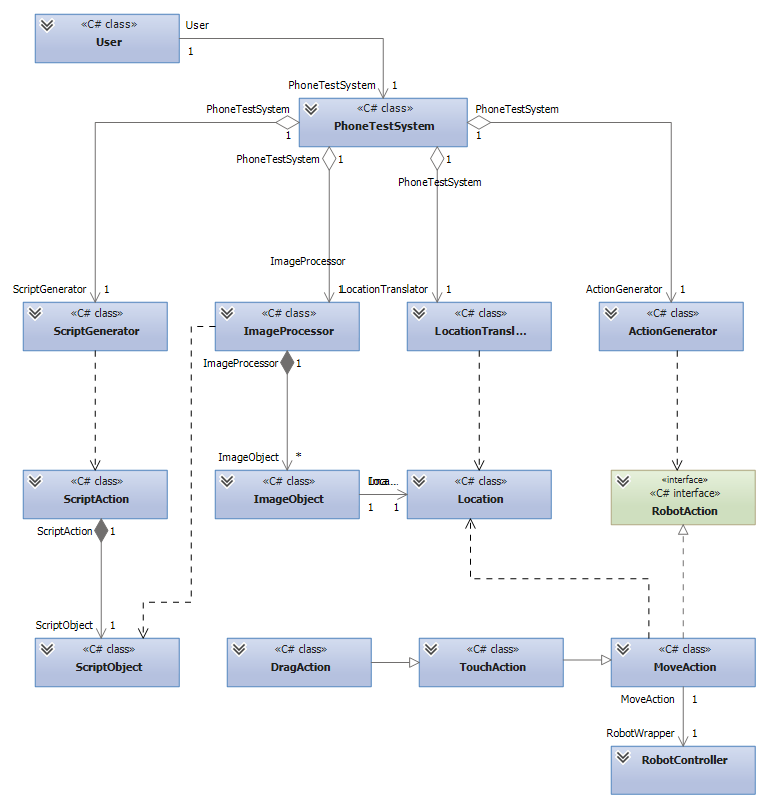
\includegraphics[scale=0.75]{Chapters/Fig/class_diagram.png}
		\caption{System class diagram}
		\label{fig:class_diagram}
	\end{figure}

\subsection{Main components of the system}
The system consists of 3 main modules, which are Image Processing module, Script Managing module and Robot Action Handling module. The image processing module is involved in detecting and recognizing screen elements along with organizing and managing them for further access. The script managing module operates the test cases. The robot handling module defines the movements of the robot and proposes inducing methods to other components so as to have the robot working.

	\begin{figure}[H]
		\centering
		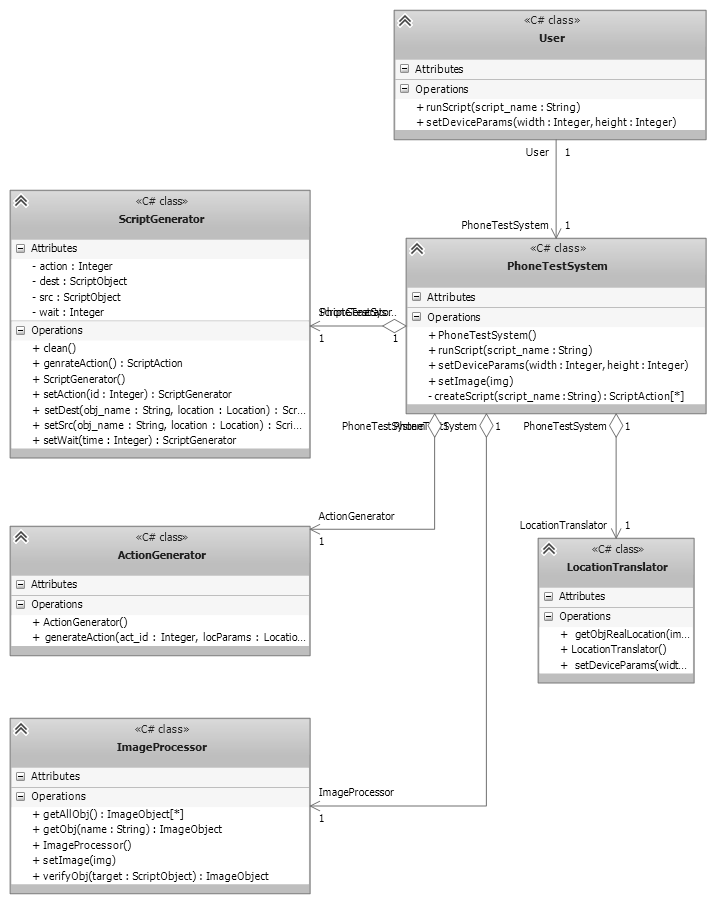
\includegraphics[scale=0.75]{Chapters/Fig/main_class.png}
		\caption{System main components}
		\label{fig:main_class}
	\end{figure}

There are also some assisting classes. PhoneTestSystem takes responsibility for wrapping up all modules and provides interface functions to the user. LocationTranslator holds user input parameters with the purpose of converting actual phone screen location into the pixel location in the screen image and vice versa.

\subsection{Image Processor structure}
Using image processing techniques presented in Chapter \ref{ch:screen_recognize}, screen elements are wrapped in objects which have names and location relative to the screen reference system.

	\begin{figure}[H]
		\centering
		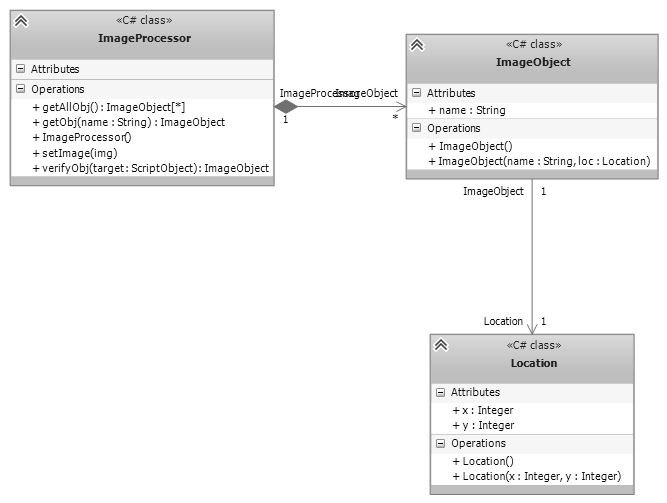
\includegraphics[scale=0.75]{Chapters/Fig/img_processor.png}
		\caption{Image Processor structure}
		\label{fig:img_processor}
	\end{figure}

An Image Processor receives image input from other classes and parses its content into a list of managed objects called Image Objects. An ImageObject holds the target's name which is text read from the screen, and location in percent with screen coordinate. The location can be converted into a real location later via LocationTranslator mentioned above. The name of the object is used for searching and verifying element in script through \textit{getObj} and \textit{verifyObj} methods of Image Processor.

\subsection{Script Generator structure}
A script is formed of sequence of actions which are introduced in Section \ref{sec:script_comp}. Considering that each action can have different members, but shares some required factors, ScriptGenerator is inspired by ``Builder Pattern'' \footnote{Read more at: \url{http://www.oodesign.com/builder-pattern.html}} to allow a dynamic way to generate script action on demand.

	\begin{figure}[H]
		\centering
		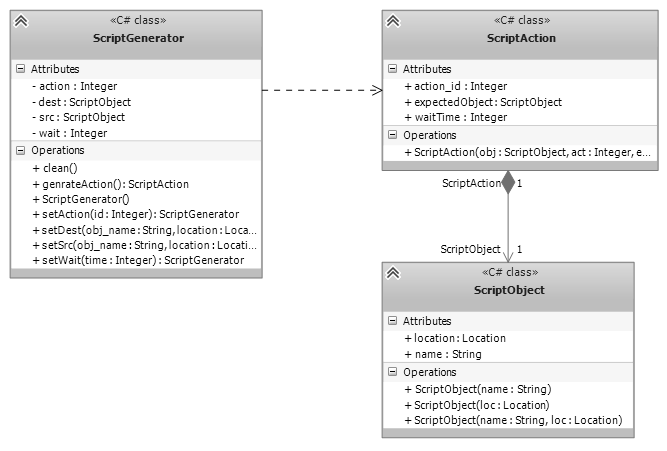
\includegraphics[scale=0.75]{Chapters/Fig/script_gen.png}
		\caption{Script Generator structure}
		\label{fig:script_gen}
	\end{figure}

Corresponding to each attribute of a script action, there is a \textit{set} method. Depending on situation, appropriate method is called. For an example, in Figure \ref{fig:click_test_diag}, a simple action like Clicking on READY button only needs a target and an action type (click, in this case). Thus, two methods ``setSrc'' and ``setAction'' are called and finished with ``generateAction'' method to produce an instance of ScriptAction. Another case is Clicking on SUCCESS button. This action requires a result to be verified which is READY button. Hence, destination object needs to be set by ``setDest'' method before ``generateAction'' being called. By using this kind of pattern, attributes of desired object are built intentionally.

\subsection{Action Generator structure}
Action Generator is in charge of providing an interface for telling the robot what to do. The actions of the robot are represented in 3 basic classes. Figure \ref{fig:act_gen} describes the relation between these classes.

	\begin{figure}[H]
		\centering
		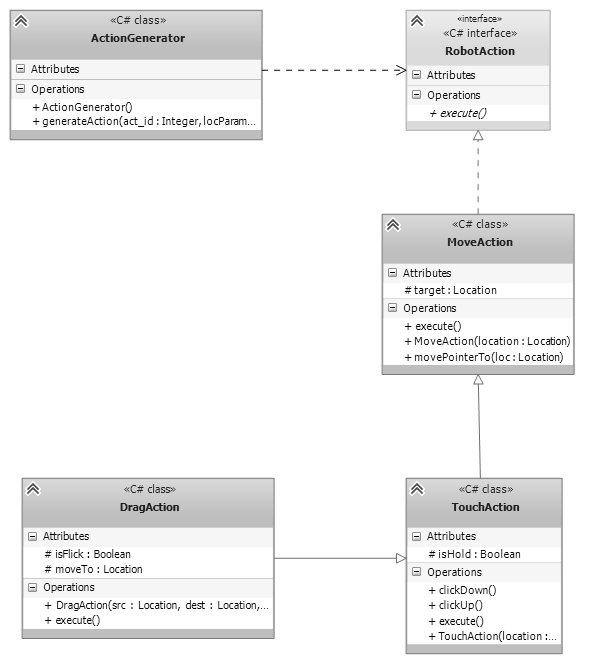
\includegraphics[scale=0.75]{Chapters/Fig/act_gen.png}
		\caption{Action Generator structure}
		\label{fig:act_gen}
	\end{figure}

Based on ``Command Pattern'' \footnote{Read more at: \url{http://www.oodesign.com/command-pattern.html}}, action request is encapsulated in an object that allows the parameterization with different requests. The client simply calls \textit{execute} method of a RobotAction instance and let the action run itself. The execution detail is predefined at action's initialization through ActionGenerator.

The most basic movement is moving the robot's pointer. When this action is executed, the pointer will be moved to the specified location. The following actions, such as Touch, Drag, Long Click and Flick, are derived from this action and then compose more complex movements.

\section{Robot interface commands}
When an action's execute method is invoked, it sends a moving command to Robot Controller. Robot Controller works like a black box. What outside clients see are high-level abstract methods. These methods include:

	\begin{itemize}
		\item[--] \textbf{Calibrate}: set the robot's pointer to initial location which is supposed to be the origin point in coordination system.
		\item[--] \textbf{GotoXYZ}: most basic function, drive the pointer to any location in 3-D space.
		\item[--] \textbf{GotoTarget}: derived from GotoXYZ, move the pointer around phone screen's area.
		\item[--] \textbf{ClickUp}, \textbf{ClickDown}: also derived from GotoXYZ, simply make the pointer up or down correspondingly.
	\end{itemize}

Without assembly intervention to the robot, the system can still interact and dictate the robot fluently under the control of a singleton class Robot Controller. By applying ``Singleton Pattern'' \footnote{Read more at: \url{http://www.oodesign.com/singleton-pattern.html}}, the robot's activities is well-handled in a form of queue and thus avoid the interference of simultaneous commands.